% =====================================================================
%  Introduction to Deep Learning — Class 23
%  Topic (course plan): Convolution Networks
%  Subtopic (course plan): Convolution Filters
%  Sources (course plan): Prince Chapter 10, Bishop Chapter 10
%
%  Class 18 listed four ways to obtain an invariance and said the fourth
%  was to build it into the architecture.  This class carries that out.
%  It is about a LAYER, not about any particular network: Class 24 is
%  the three tasks, Class 25 is depth, architectures and what the
%  filters learn.
%
%  Order: why a dense layer is impossible, what invariance and
%  equivariance demand, the operation in one dimension and its three
%  knobs, channels and receptive fields, two dimensions, and changes of
%  resolution.
%
%  Two results are stated in neither textbook; the C variant is this
%  deck with those two removed.  See _shared/PLAN_Classes23_24_25.md.
%
%  Compile:  xelatex main.tex   (run twice)
% =====================================================================
\documentclass[aspectratio=169, 11pt]{beamer}

\usetheme{metropoliscustom}

\usepackage{graphicx}
\DeclareGraphicsExtensions{.pdf,.png,.jpg}
\graphicspath{{figs/}{Class23_Convolution_Filters/B_Recreated_Figures/figs/}}
\usepackage{amsmath, amssymb}
\usepackage{bm}
\usepackage{tikz}
\usetikzlibrary{arrows.meta, positioning, calc, decorations.pathreplacing,
                shapes.geometric, fit, backgrounds}
\tcbuselibrary{skins}

\definecolor{shc}{HTML}{341651}
\definecolor{tealc}{HTML}{1C7293}
\definecolor{dpc}{HTML}{800000}
\definecolor{accc}{HTML}{B8860B}

% ---- theorem environments -------------------------------------------
\setbeamertemplate{theorems}[numbered]
\usepackage{remreset}
\makeatletter\@removefromreset{theorem}{section}\makeatother
\renewcommand{\thetheorem}{\arabic{theorem}}
\newtheorem{lemmax}[theorem]{Lemma}
\newtheorem{propx}[theorem]{Proposition}
\newtheorem{corx}[theorem]{Corollary}
\newtheorem{defx}[theorem]{Definition}
\newtheorem{thmx}[theorem]{Theorem}

\newcommand{\bridge}[1]{%
  {\scriptsize\itshape\color{mcMuted} #1\par}\vspace{0.35em}}

\newcommand{\srcline}[1]{%
  \par\vspace{0.25em}%
  {\scriptsize\color{mcMuted}\hfill #1\par}}

\newcommand{\figsource}[1]{{\scriptsize\color{mcMuted} #1}}
\newcommand{\figcap}[2][0.90]{%
  \begin{center}\begin{minipage}{#1\textwidth}\centering
    {\scriptsize\color{mcMuted} #2}
  \end{minipage}\end{center}}

% =====================================================================
\title{Convolutional Networks}
\subtitle{Convolution Filters}
\author{Introduction to Deep Learning \ \textperiodcentered\ }
\institute{}
\date{}

\footleft{Introduction to Deep Learning}
\footright{Convolution Filters}
\titlelogos{}

\begin{document}

\maketitle

\begin{frame}{Outline}
  \tableofcontents
\end{frame}

% =====================================================================
\section{Why Not a Dense Layer}
% =====================================================================

\begin{frame}{Building the symmetry in, rather than learning it}
  \bridge{Class 18 listed four ways to obtain an invariance and said the
  fourth was to build it into the architecture. This class carries that
  out.}
  \vspace{0.15em}
  {\scriptsize
  \renewcommand{\arraystretch}{1.24}
  \begin{tabular}{@{}l@{\hspace{1.3em}}l@{\hspace{1.3em}}l@{}}
    \textbf{Route to an invariance} & \textbf{What it costs} & \textbf{Class}\\
    pre-processing & may discard useful information & 18\\
    a penalty on output change & only small transformations & 18\\
    augmentation & more data, more compute & 19\\
    \textbf{the architecture} & \textbf{the symmetry must be known} &
      \textbf{today}\\
  \end{tabular}}
  \vspace{0.5em}

  \begin{redhighlight}
    Today is about one layer, not about any network. What you build with
    it is Class 24; how deep to stack it, and what the filters end up
    detecting, is Class 25.
  \end{redhighlight}
\end{frame}

\begin{frame}{Notation for today}
  \vspace{0.35em}
  {\footnotesize
  \renewcommand{\arraystretch}{1.30}
  \begin{columns}[T, onlytextwidth]
    \begin{column}{0.49\textwidth}
      \begin{tabular}{@{}l@{\hspace{1.4em}}l@{}}
        $\mathbf{x}$, $\mathbf{z}$ & input and output of a layer\\
        $\mathbf{w}$ & the \alert{kernel}, of size $k$\\
        $i$, $j$ & spatial positions\\
        $c$, $c'$ & input and output channels\\
      \end{tabular}
    \end{column}
    \begin{column}{0.49\textwidth}
      \begin{tabular}{@{}l@{\hspace{1.4em}}l@{}}
        $s$ & stride\\
        $d$ & dilation rate\\
        $p$ & padding width\\
        $r_l$ & receptive field after $l$ layers\\
      \end{tabular}
    \end{column}
  \end{columns}}
  \vspace{0.55em}

  \begin{itemize}\itemsep0.24em
    \item Bishop says \emph{filter} and Prince says \emph{kernel} for the
          same object; this deck says kernel
    \item What both books call convolution is, strictly,
          \alert{cross-correlation}: the kernel is not flipped. The
          convention is universal and harmless, since the weights are
          learned either way
  \end{itemize}
  \srcline{Prince (2023), Eq.~10.3 and its footnote; Bishop \& Bishop
  (2024), Eq.~10.1.}
\end{frame}


\begin{frame}{Images as Data}
  \vspace{-0.15em}
  \begin{block}{The cost of a dense first layer}
    \small
    A colour image of $10^3 \times 10^3$ pixels has $3 \times 10^6$
    inputs. A fully connected first layer with $1{,}000$ hidden units
    therefore has $3 \times 10^{9}$ weights --- in the first layer alone.
    A convolutional layer with $64$ channels and a $3\times3$ kernel has
    $3 \times 3 \times 3 \times 64 + 64 = 1{,}792$, whatever the image
    size.
  \end{block}
  \vspace{0.3em}
  {\footnotesize
  \begin{itemize}\itemsep0.22em
    \item The dense layer also has to \alert{learn} that a cat is still a
          cat one pixel to the left, from examples
    \item And it treats the pixels as unstructured: permute them and the
          layer is unchanged, while the image is destroyed
    \item Nearby pixels are strongly correlated, and that is prior
          knowledge worth building in
  \end{itemize}}
  \srcline{Bishop \& Bishop (2024), \S10.1.1 and \S10.2;
  Prince (2023), \S10.2.4.}
\end{frame}

\begin{frame}{Images as Data}
  \vspace{-0.5em}
  \begin{center}
    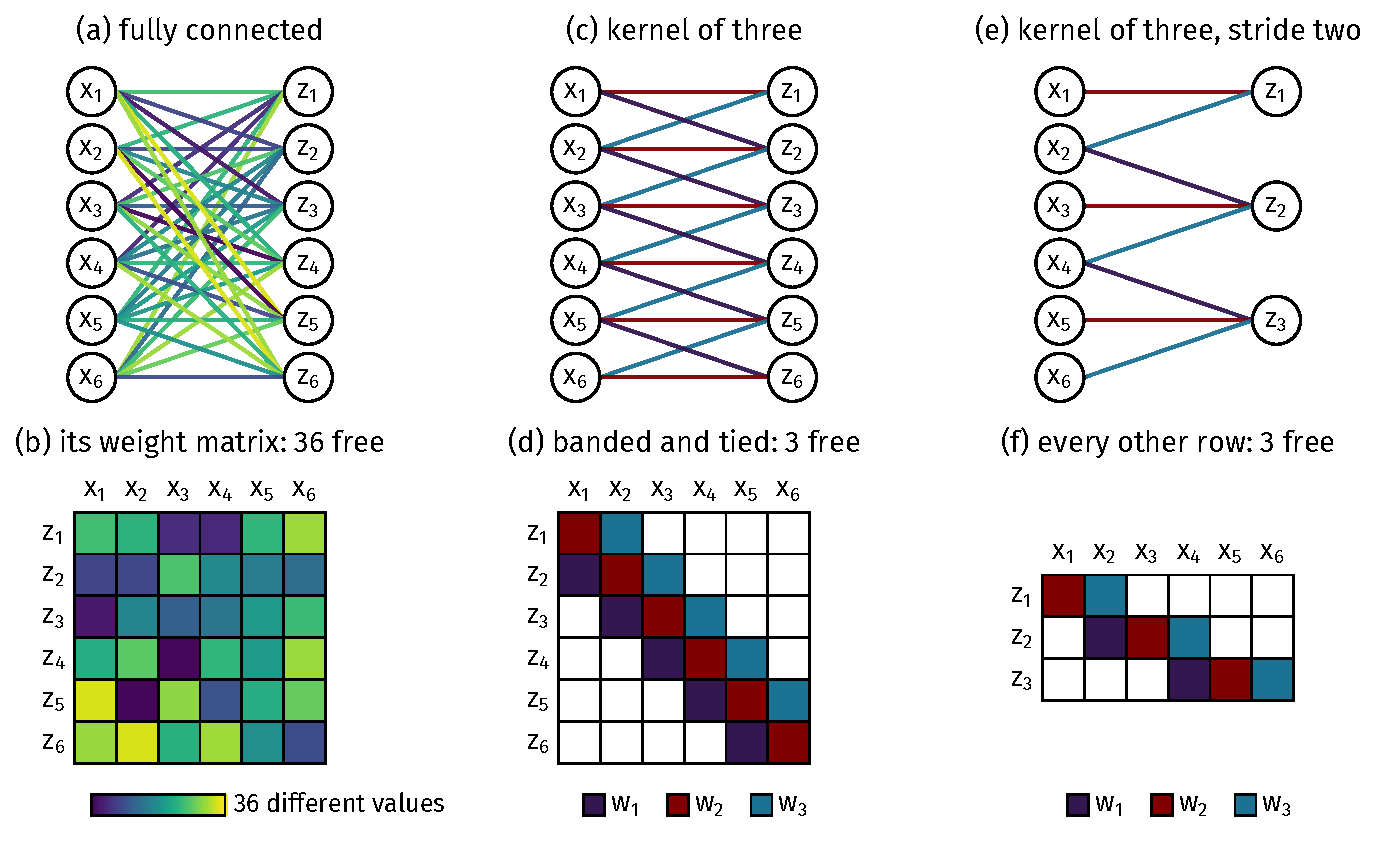
\includegraphics[width=0.69\linewidth]{dense_vs_conv}
  \end{center}
  \vspace{-0.8em}
  {\tiny\color{mcMuted}
  (a--b) a fully connected layer on six inputs: every one of the $36$
  weights is free. (c--d) a convolutional layer with kernel three: most
  entries are zero and the rest repeat, so three numbers describe the
  whole matrix. (e--f) the same with stride two.
  \hfill Prince (2023), Fig.~10.4.\par}
\end{frame}

% =====================================================================
\section{Invariance and Equivariance}
% =====================================================================
\begin{frame}{Images}
  \begin{center}
    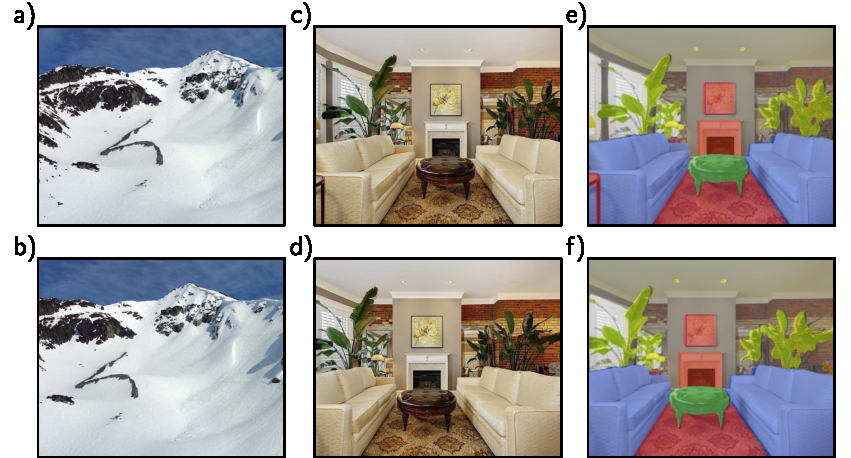
\includegraphics[height=0.505\textheight]{P_ConvEquiInv}
  \end{center}
  \figcap[0.97]{(a--b) classification: the horizontal shift must leave
  the label ``mountain'' unchanged --- invariance. (c--f) segmentation:
  when the image is translated, the per-pixel output must translate with
  it --- equivariance. Prince (2023), Fig.~10.1.}
\end{frame}

\begin{frame}{Some Definitions}
  \vspace{-0.2em}
  \begin{defx}[Invariance and equivariance]\label{th:inv}
    \small
    For a transformation $t[\cdot]$ of the input, a function $f$ is
    \alert{invariant} if
    \[
      f\big[t[\mathbf{x}]\big] = f[\mathbf{x}],
      \qquad\text{and \alert{equivariant} if}\qquad
      f\big[t[\mathbf{x}]\big] = t\big[f[\mathbf{x}]\big].
    \]
  \end{defx}
  \vspace{0.3em}
  {\footnotesize
  \begin{itemize}\itemsep0.22em
    \item Classify an image: translate it and the label must not move
          --- invariance
    \item Segment an image: translate it and the mask must move with it
          --- equivariance
    \item A network gets invariance by making its \emph{layers}
          equivariant and then discarding position at the end
  \end{itemize}}
  \srcline{Prince (2023), Eqs.~10.1--10.2, Fig.~10.1;
  Bishop \& Bishop (2024), \S10.2.2.}
\end{frame}



% =====================================================================
\section{The Operation}
% =====================================================================
\begin{frame}{One dimension, one kernel}
  \vspace{-0.5em}
  \begin{center}
    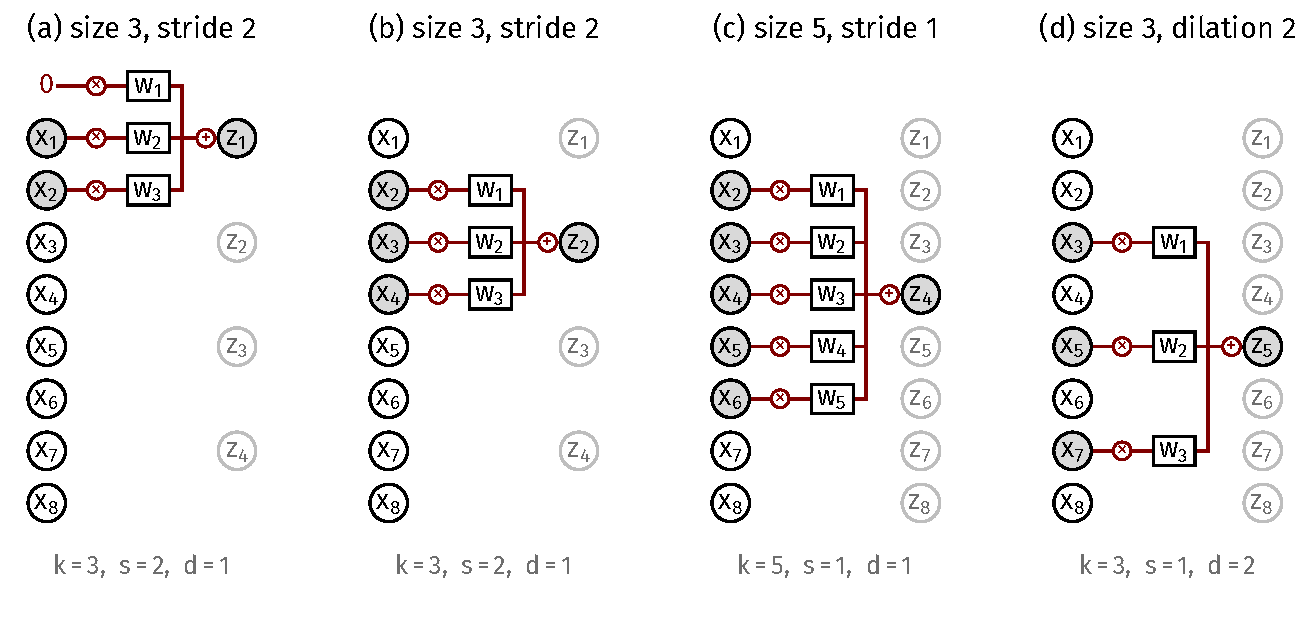
\includegraphics[width=0.86\linewidth]{conv_knobs}
  \end{center}
  \vspace{-0.8em}
  {\tiny\color{mcMuted}
  Eight inputs each time; shaded inputs are the ones the shaded output
  reads, through the weights $w_j$. (a--b) stride two evaluates the
  kernel at every other position, and $z_1$ reads a zero pad. (c) a
  kernel of five reads more and costs more weights. (d) a dilated kernel
  reaches as far as a kernel of five wit
  \hfill Prince (2023), Fig.~10.3.\par}
\end{frame}
\begin{frame}{Three knobs, and one formula}
  \vspace{-0.15em}
  \begin{propx}[Output length]\label{th:size}
    \small
    A 1-D convolution with kernel size $k$, stride $s$, dilation $d$ and
    zero padding $p$ on an input of length $n$ produces
    \[
      n_{\mathrm{out}}
        \;=\; \Big\lfloor \frac{n + 2p - d(k-1) - 1}{s} \Big\rfloor + 1 .
    \]
    The dilated kernel spans $d(k-1)+1$ positions while using only $k$
    weights.
  \end{propx}
  \vspace{0.25em}
  {\footnotesize
  \begin{itemize}\itemsep0.20em
    \item \alert{Padding} decides whether the representation shrinks at
          the edges; %\emph{valid} padding invents nothing but loses size
    \item \alert{Stride} subsamples the output; \alert{dilation} widens
          the reach without buying more weights
  \end{itemize}}
  \srcline{Prince (2023), \S10.2.2--10.2.3, Fig.~10.3;
  Bishop \& Bishop (2024), \S10.2.3--10.2.4; Dumoulin \& Visin (2016).}
\end{frame}
\begin{frame}{One dimension, one kernel}
  \vspace{-0.35em}
  \[
    z_i \;=\; \sum_{j=1}^{k} w_j\, x_{\,i + j - \lceil k/2 \rceil},
    \qquad
    h_i \;=\; a\Big[\beta + \sum_{j=1}^{k} w_j\, x_{\,i+j-2}\Big]
    \quad (k = 3).
  \]
  \vspace{-0.45em}
  {\footnotesize
  \begin{itemize}\itemsep0.24em
    \item Each output reads a window of $k$ inputs. The same $k$ weights
          are used at \alert{every} position --- this is the parameter
          sharing, in its canonical form
    \item A convolutional layer adds a bias and an activation, exactly
          as a dense layer does
    \item Compare a dense layer, $h_i = a[\beta_i + \sum_{j=1}^{D}
          \Omega_{ij} x_j]$: $D^2$ weights and $D$ biases against
          $k$ weights and one bias
  \end{itemize}}
  \srcline{Prince (2023), Eqs.~10.3--10.5, Figs.~10.2, 10.4.}
\end{frame}

\begin{frame}{A convolution is a dense layer with most of it deleted}
  \begin{center}
    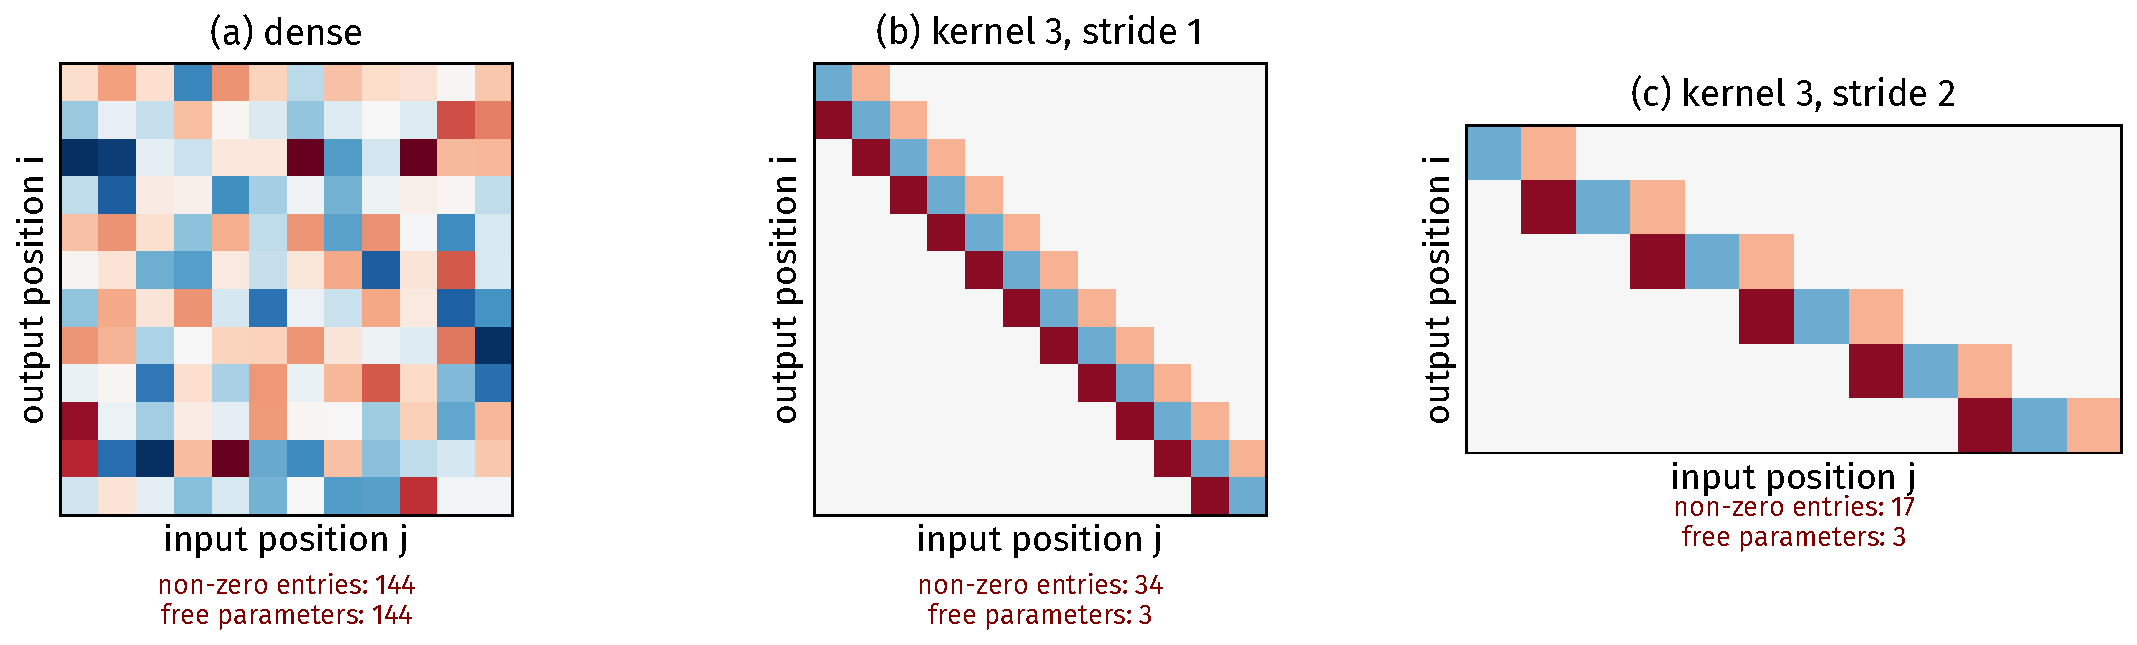
\includegraphics[width=0.94\linewidth]{weight_matrix}
  \end{center}
  % \figcap[0.97]{The actual matrix each layer applies, on twelve inputs.
  % (a) dense: $144$ free numbers. (b) kernel three: $34$ non-zeros but
  % only \alert{three} free numbers, because the colours repeat down the
  % band. (c) stride two removes every other row. Sparsity alone would
  % leave $3n$ free weights; tying them is what leaves three.}
\end{frame}





\begin{frame}{What one kernel responds to}
  \vspace{-0.2em}
  \begin{propx}[The kernel is what it detects]\label{th:matched}
    \small
    For a unit $z = \mathrm{ReLU}(\mathbf{w}^{\mathsf T}\mathbf{x} + w_0)$ acting on a
    patch $\mathbf{x}$ of fixed norm, the patch maximising the response is
    $\mathbf{x} = \gamma\,\mathbf{w}$ for some $\gamma > 0$. So the unit fires
    hardest on the patch that \alert{looks like its own kernel}, and the
    bias sets how good a match is good enough.
  \end{propx}
  \vspace{0.25em}
  {\footnotesize
  \begin{itemize}\itemsep0.22em
    \item One line, by Cauchy--Schwarz:
          $\mathbf{w}^{\mathsf T}\mathbf{x} \leq \|\mathbf{w}\|\,\|\mathbf{x}\|$ with
          equality only when $\mathbf{x}$ is parallel to $\mathbf{w}$
    \item This is why a kernel can be drawn as a small image and read as
          a template
    \item What templates a trained network settles on is Class 25
  \end{itemize}}
  \srcline{Bishop \& Bishop (2024), \S10.2.1, Eq.~10.1, Exercise 10.1.}
\end{frame}
\begin{frame}{Convolution is the equivariant linear map}
  \vspace{-0.25em}
  \begin{thmx}[Equivariance, and its converse]\label{th:equi}
    \small
    Let $T_a$ shift a signal by $a$ positions. A convolution
    $z_i = \sum_j w_j\, x_{i+j}$ satisfies
    $\mathrm{conv}(T_a \mathbf{x}) = T_a\,\mathrm{conv}(\mathbf{x})$ for every $a$.
    Conversely, a linear map $\mathbf{z} = \bm{\Omega}\mathbf{x}$ that commutes
    with every $T_a$ must have $\Omega_{ij}$ depending only on $i-j$ ---
    that is, it \alert{is} a convolution.
  \end{thmx}
  \vspace{0.25em}
  {\footnotesize
  % \begin{itemize}\itemsep0.22em
  %   \item So convolution is not one convenient equivariant layer among
  %         many. Up to boundary handling it is the \alert{only} linear one
  %   \item The forward direction is the reason to use it; the converse is
  %         the reason there is nothing else to try
  % \end{itemize}
  }
  \srcline{Bishop \& Bishop (2024), \S10.2.2; converse from
  Cohen \& Welling (2016).}
\end{frame}

\begin{frame}{Proof, in both directions}
  \vspace{-0.25em}
  {\footnotesize
  \begin{itemize}\itemsep0.28em
    \item \focus{1}{Forward. Write $y_i = (T_a \mathbf{x})_i = x_{i-a}$. Then
          $\mathrm{conv}(\mathbf{y})_i = \sum_j w_j\, y_{i+j}
          = \sum_j w_j\, x_{i-a+j}$.}
    \item \focus{1}{That last expression is exactly
          $\mathrm{conv}(\mathbf{x})_{i-a}$, which is
          $T_a\,\mathrm{conv}(\mathbf{x})$ evaluated at $i$. \hfill $\square$}
    \item \focus{1}{Converse. Commuting with $T_a$ means
          $\bm{\Omega} T_a = T_a \bm{\Omega}$ for every $a$, and in
          coordinates that reads
          $\Omega_{i,\,j+a} = \Omega_{i-a,\,j}$.}
    \item \focus{1}{Setting $a = -c$, $j=c$ and $i=r-c$ gives
          $\Omega_{r-c,0} = \Omega_{r,\,c}$, so every entry is fixed by
          the single index $r-c$ (or $i-j)$.}
    \item \focus{1}{Define $w_{i-j} = \Omega_{ij}$. Then
          $z_i = \sum_j \Omega_{ij} x_j = \sum_j w_{i-j} x_j$, a
          convolution. \hfill $\square$}
  \end{itemize}}
  \vspace{-0.15em}
  \begin{redhighlight}
    Sharing the weights is not a trick to save memory. It is what
    equivariance forces, and the saving is a consequence.
  \end{redhighlight}
\end{frame}

% =====================================================================
\section{Channels, Layers and Receptive Fields}
% =====================================================================

\begin{frame}{One kernel is not enough}
  \vspace{-0.3em}
  \[
    h^{c'}_{i}
      \;=\; a\Big[\beta_{c'} \;+\;
        \sum_{c=1}^{C_{\mathrm{in}}}\ \sum_{j=1}^{k}
          \Omega_{c,\,c',\,j}\; x^{c}_{\,i+j-2}\Big] ,
    \qquad
    \bm{\Omega} \in \mathbb{R}^{C_{\mathrm{in}} \times C_{\mathrm{out}} \times k} .
  \]
  \vspace{-0.4em}
  {\footnotesize
  \begin{itemize}\itemsep0.24em
    \item A single convolution averages and then clips, so information
          is lost. Several are run in parallel, and each output is a
          \alert{channel} or \alert{feature map}
    \item Every output channel reads \emph{all} input channels over
          $k$ positions, so the layer has
          $C_{\mathrm{in}} C_{\mathrm{out}} k$ weights and
          $C_{\mathrm{out}}$ biases
    \item Still independent of the length of the input
  \end{itemize}}
  \srcline{Prince (2023), \S10.2.5, Fig.~10.5.}
\end{frame}

\begin{frame}{How far back a unit can see}
  \vspace{-0.2em}
  \begin{thmx}[Receptive field]\label{th:rf}
    \small
    Stack layers with kernel sizes $k_1, \dots, k_L$ and strides
    $s_1, \dots, s_L$. The number of input positions feeding one unit of
    layer $l$ is
    \[
      r_0 = 1, \qquad
      r_l \;=\; r_{l-1} \;+\; (k_l - 1)\prod_{j<l} s_j .
    \]
    With all strides one this is $r_l = 1 + l\,(k-1)$: linear in depth.
    With stride two everywhere the product doubles each layer, so $r_l$
    grows \alert{exponentially}.
  \end{thmx}
  \vspace{0.2em}
  {\footnotesize
  \begin{itemize}\itemsep0.20em
    \item A unit that has not seen a pixel cannot depend on it, so the
          receptive field is the budget within which any feature must
          fit
  \end{itemize}}
  \srcline{Prince (2023), \S10.2.6, Fig.~10.6; Luo et al.\ (2016).}
\end{frame}

\begin{frame}{The recursion, checked}
  \begin{center}
    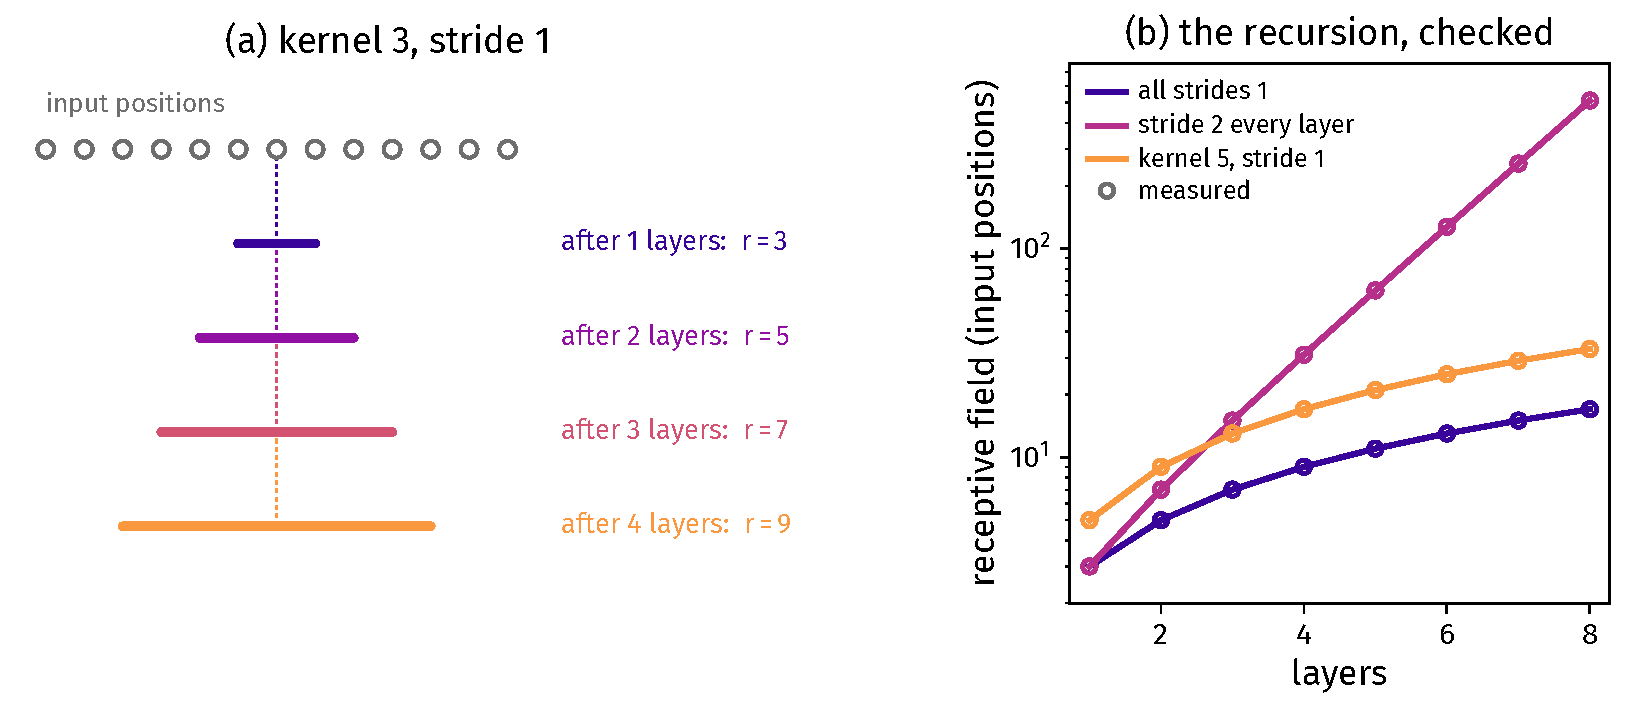
\includegraphics[width=0.70\linewidth]{receptive_field}
  \end{center}
  \figcap[0.97]{(a) the span reaching one unit after one to four layers
  of kernel three and stride one: $3, 5, 7, 9$. (b) the recursion
  (lines) against the field measured by propagating a single one back
  through the stack (markers), for three schedules. They agree at every
  depth.}
\end{frame}

\begin{frame}{How far back a unit can see, drawn}
  \vspace{-0.4em}
  \begin{center}
    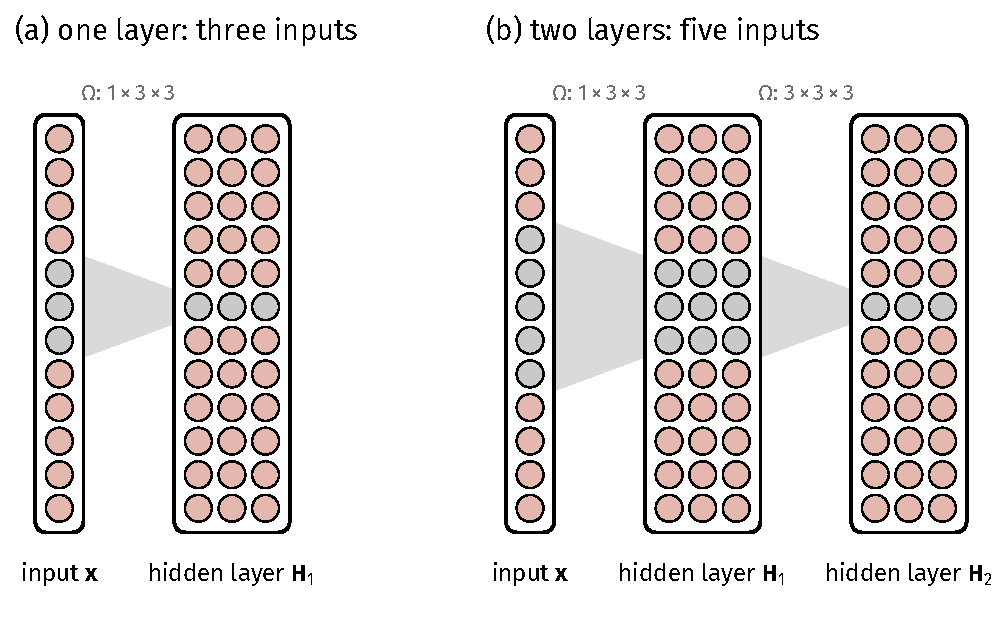
\includegraphics[width=0.65\linewidth]{rf_spot_ab}
  \end{center}
  \vspace{-0.7em}
  {\tiny\color{mcMuted}
  Each layer is a column of units, three channels wide after the input;
  grey units lie in the receptive field of the shaded row on the right,
  and the spotlight shows which units of one layer reach the next.
  (a) a unit in the first hidden layer sees three inputs. (b) one in the
  second sees five, because each of its three inputs saw three.
  \hfill Prince (2023), Fig.~10.6.\par}
\end{frame}

\begin{frame}{How far back a unit can see, drawn}
  \vspace{-0.4em}
  \begin{center}
    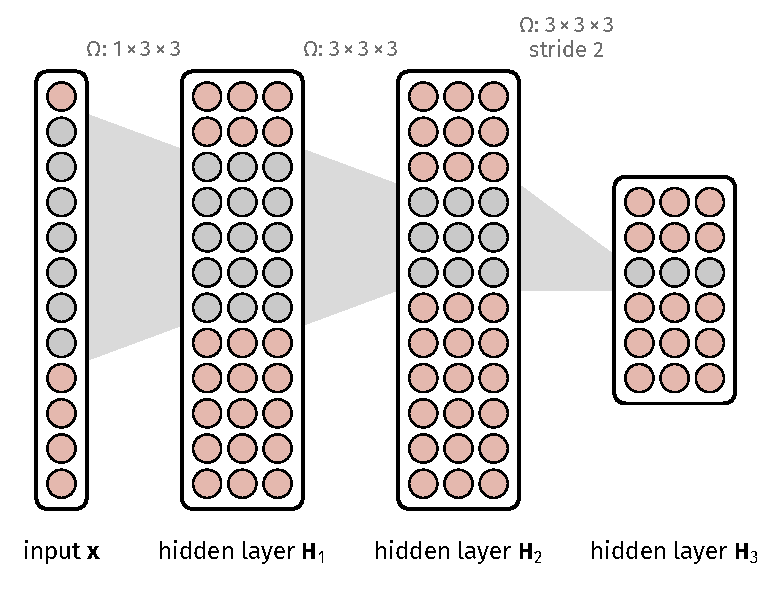
\includegraphics[width=0.53\linewidth]{rf_spot_c}
  \end{center}
  \vspace{-0.7em}
  {\tiny\color{mcMuted}
  (c) a third layer with stride two halves the number of units and
  doubles the step of every kernel after it: a unit there reaches seven
  inputs.
  \hfill Prince (2023), Fig.~10.6.\par}
\end{frame}

\begin{frame}{How far back a unit can see, drawn}
  \vspace{-0.4em}
  \begin{center}
    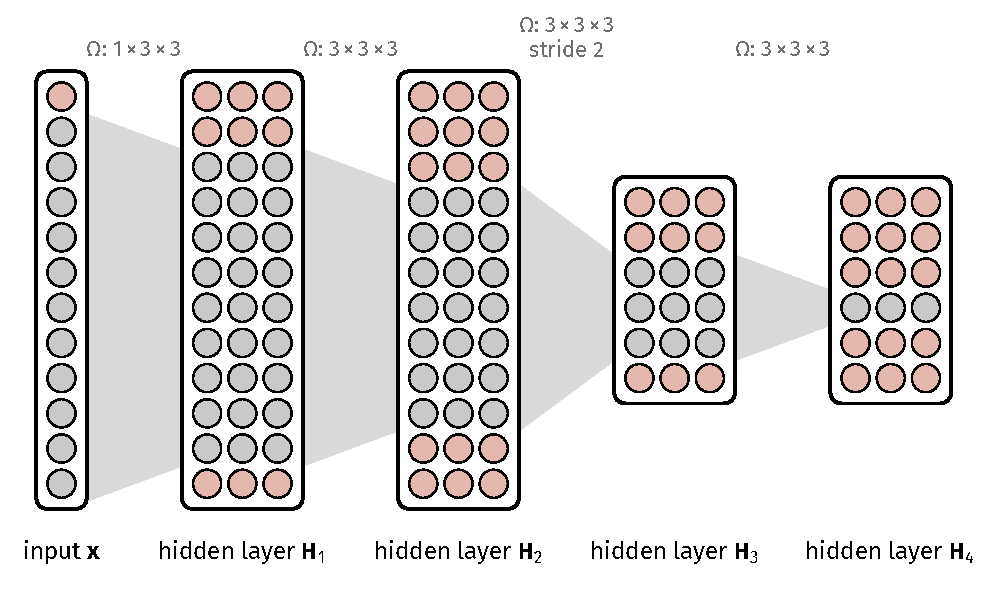
\includegraphics[width=0.66\linewidth]{rf_spot_d}
  \end{center}
  \vspace{-0.7em}
  {\tiny\color{mcMuted}
  (d) by the fourth layer the field covers eleven of the twelve inputs,
  which is what the recursion $r_4 = 7 + 2 \cdot 2$ gives; every field
  here is computed by propagation, and the build checks it against the
  recursion.
  \hfill Prince (2023), Fig.~10.6.\par}
\end{frame}

   

% =====================================================================
\section{Two Dimensions}
% =====================================================================

\begin{frame}{2D data: Images}
  \vspace{-0.35em}
  \[
    h^{c'}_{i,j}
      \;=\; a\Big[\beta_{c'} + 
        \sum_{u=1}^{k}\sum_{v=1}^{k}
        \Omega_{c,c',u,v}\; x^{c}_{\,i+u-2,\; j+v-2}\Big]
  \]
  \vspace{-0.4em}
  {\footnotesize
  \begin{itemize}\itemsep0.22em
    \item Nothing conceptual changes: the window is a square, the
          weights are still shared across positions, and the layer is
          still equivariant --- now to translations in two directions
    \item Parameters: $k^2 C_{\mathrm{in}} C_{\mathrm{out}} +
          C_{\mathrm{out}}$. For $k=3$, $C_{\mathrm{in}} =
          C_{\mathrm{out}} = 64$: $36{,}928$, whatever the image size
    \item A $1\times1$ convolution mixes channels and nothing else,
          which is how the channel count is changed cheaply
  \end{itemize}}
  \srcline{Prince (2023), \S10.3, Eq.~10.6, Figs.~10.8--10.10;
  Bishop \& Bishop (2024), \S10.2.5.}
\end{frame}

\begin{frame}{2D Convolution}
 \vspace{-0.5cm}
 \begin{center}
 
\includegraphics[scale=0.55]{Class23_Convolution_Filters/B_Recreated_Figures/figs/Deep Learning.JPG}  \vspace{-0.5cm}
\srcline{Prince (2023), \S10.3, Eq.~10.6, Fig.~10.9;
  Bishop \& Bishop (2024), \S10.2.5.}
  \end{center}
\end{frame}

\begin{frame}{2D Convolution with Color Images}
 \vspace{-0.5cm}
 \begin{center}
 
\includegraphics[scale=0.65]{Class23_Convolution_Filters/B_Recreated_Figures/figs/3D_color.JPG}  \vspace{-0.5cm}
   \[
    h^{c'}_{i,j}
      \;=\; a\Big[\beta_{c'} + \sum_{c=1}^{C_{\mathrm{in}}}
        \sum_{u=1}^{k}\sum_{v=1}^{k}
        \Omega_{c,c',u,v}\; x^{c}_{\,i+u-2,\; j+v-2}\Big]
  \]
\srcline{Prince (2023), \S10.3, Eq.~10.6, Fig.~10.10;
  Bishop \& Bishop (2024), \S10.2.5.}
  \end{center}
\end{frame}

\begin{frame}{What a $3 \times 3$ kernel does}
  \begin{center}
    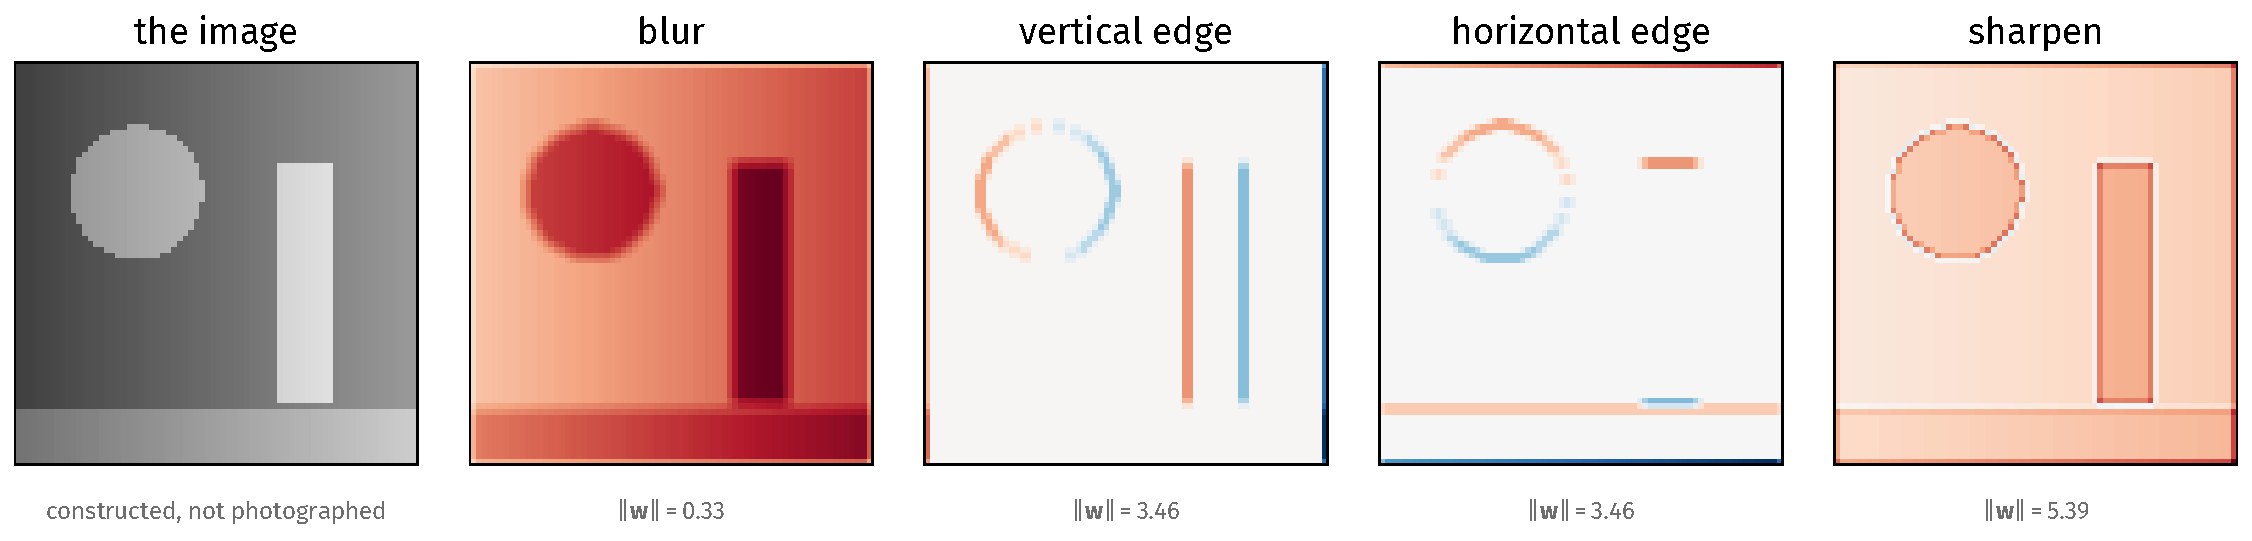
\includegraphics[width=0.96\linewidth]{kernels_2d}
  \end{center}
  \figcap[0.97]{The same nine weights applied at every position of a
  constructed scene. The edge kernels respond only where the intensity
  changes, and only in the direction they were built for --- which is
  Proposition~\ref{th:matched} seen from the other side. These four are
  hand-chosen; a network learns its own.}
\end{frame}

\begin{frame}{What a $3 \times 3$ kernel does, on an image}
  \begin{center}
    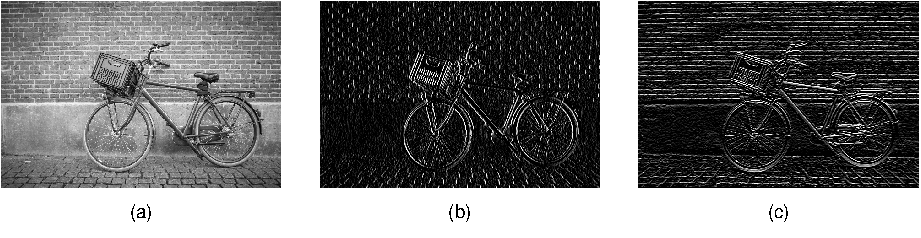
\includegraphics[width=0.90\linewidth]{Bishop10_4}
  \end{center}
  \figcap[0.97]{(a) the original image. (b) the output of a filter that
  responds to vertical edges. (c) the output of one that responds to
  horizontal edges. The same small kernel is applied at every position.
  Bishop \& Bishop (2024), Fig.~10.4.}
\end{frame}

% =====================================================================
\section{Changing Resolution}
% =====================================================================

\begin{frame}{Down, and back up}
  \vspace{-0.15em}
  {\scriptsize
  \renewcommand{\arraystretch}{1.22}
  \begin{tabular}{@{}l@{\hspace{1.2em}}l@{\hspace{1.2em}}l@{}}
    \textbf{Downsampling} & \textbf{Keeps} & \textbf{Note}\\
    max pooling & the strongest response in each window &
      no parameters\\
    mean pooling & the average of each window & no parameters\\
    strided convolution & a learned summary & has parameters\\[0.4em]
    \textbf{Upsampling} & \textbf{Fills in with} & \textbf{Note}\\
    duplication & the nearest value & no parameters\\
    zero insertion & zeros, then a convolution &
      \emph{transposed} convolution\\
    max unpooling & the value at the remembered argmax &
      needs the indices\\
    bilinear & a linear interpolation & no parameters\\
  \end{tabular}}
  \vspace{0.4em}

  {\footnotesize
  \begin{itemize}\itemsep0.20em
    \item Pooling trades \alert{where} for \alert{whether}: tolerance to
          small shifts, bought with the ability to localise
  \end{itemize}}
  \srcline{Prince (2023), \S10.4; Bishop \& Bishop (2024), \S10.2.6.}
\end{frame}

\begin{frame}{Resolution, drawn}
  \vspace{-0.5em}
  \begin{center}
    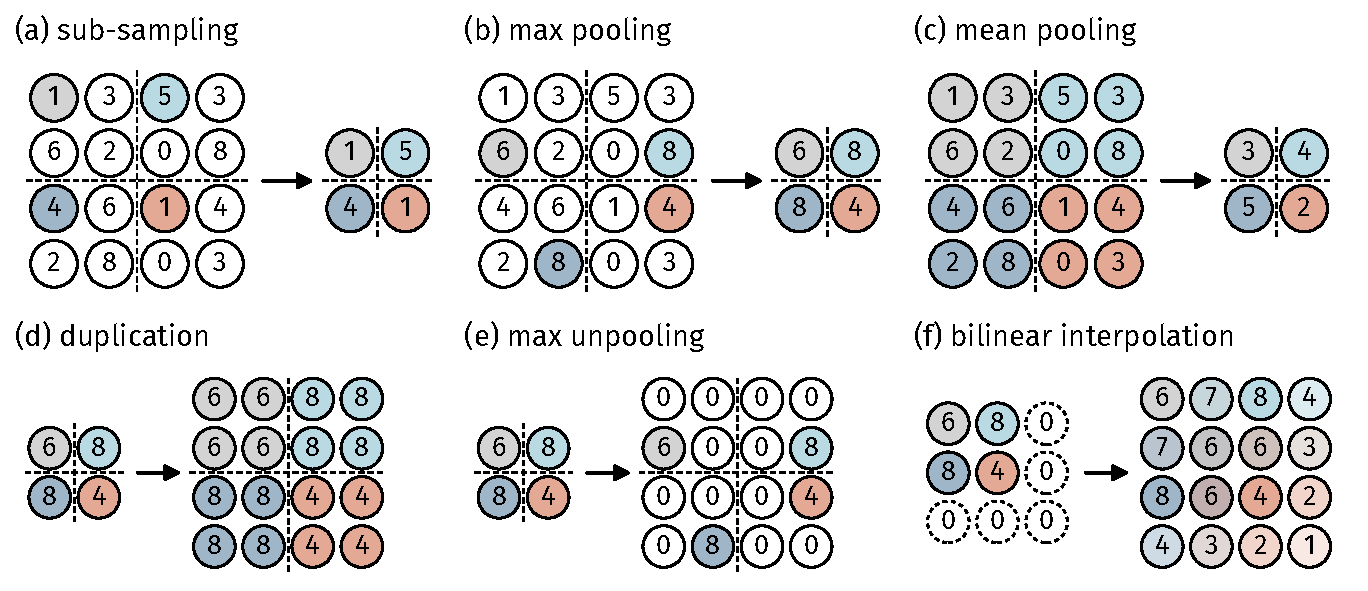
\includegraphics[width=0.92\linewidth]{resolution_circles}
  \end{center}
  \vspace{-0.8em}
  {\tiny\color{mcMuted}
  A $4 \times 4$ array, each block in its own tint; every number is
  computed. Down: (a) sub-sampling keeps one entry per block, (b) max
  pooling the largest, (c) mean pooling the average. Back up from (b):
  (d) duplication, (e) max unpooling to the remembered positions, zeros
  elsewhere, (f) bilinear interpolation, which blends the numbers and
  the tints alike.
  \hfill Prince (2023), Figs.~10.11 and 10.12.\par}
\end{frame}

\begin{frame}{Resolution, measured}
  \begin{center}
    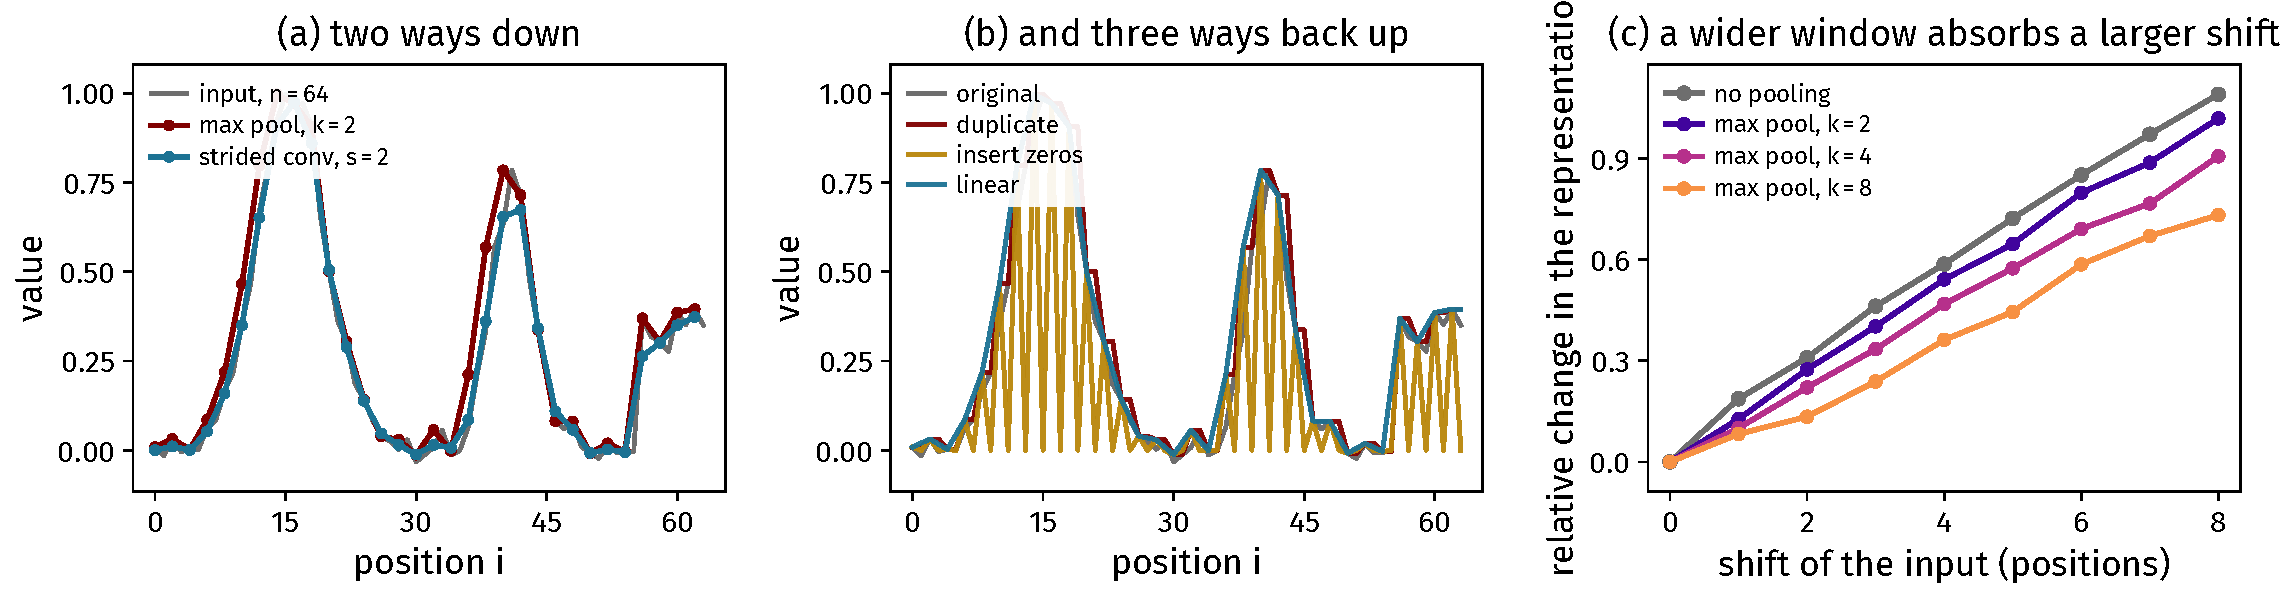
\includegraphics[width=0.96\linewidth]{resolution}
  \end{center}
  \figcap[0.97]{(a) two ways to halve a signal. (b) three ways to put it
  back: none recovers what pooling discarded, which is why an
  architecture that needs the detail keeps a copy of it. (c) translating
  the input by one position changes the raw signal by $14\%$ and an
  eight-wide pooled signal by $6\%$.}
\end{frame}

% =====================================================================
\section{Putting It Together}
% =====================================================================

\begin{frame}{The layer, in one table}
  \vspace{-0.05em}
  {\scriptsize
  \renewcommand{\arraystretch}{1.24}
  \begin{tabular}{@{}l@{\hspace{1.0em}}l@{\hspace{1.0em}}l@{}}
    \textbf{Choice} & \textbf{What it controls} & \textbf{Cost}\\
    kernel size $k$ & how much context one unit reads &
      $k$ or $k^2$ weights per channel pair\\
    stride $s$ & the output resolution &
      none; discards positions\\
    dilation $d$ & the reach, without more weights &
      gaps in what is read\\
    padding $p$ & whether the edges survive &
      invents values, or loses size\\
    channels $C_{\mathrm{out}}$ & how many features per position &
      linear in $C_{\mathrm{out}}$\\
    depth $L$ & the receptive field, and nonlinearity &
      linear in $L$\\
    pooling & tolerance to small shifts &
      the ability to localise\\
  \end{tabular}}
  \vspace{0.55em}

  \begin{redhighlight}
    Everything above is a statement about the layer. Not one of these
    choices depends on the size of the image, which is exactly the
    property the dense layer lacked.
  \end{redhighlight}
\end{frame}

\begin{frame}{Takeaways}
  \vspace{-0.05em}
  {\scriptsize
  \begin{enumerate}\itemsep0.30em
    \item A dense first layer on a $1000^2$ colour image needs
          $3 \times 10^9$ weights; a $3\times3$ convolution with $64$
          channels needs $1{,}792$, whatever the image size
          (Proposition~\ref{th:cost})
    \item Classification wants invariance and segmentation wants
          equivariance; equivariant layers plus a final discard of
          position give both (Definition~\ref{th:inv})
    \item Convolution is translation-equivariant, and every
          translation-equivariant linear map is a convolution
          (Theorem~\ref{th:equi})
    \item Weight sharing is what equivariance forces; the parameter
          saving is a consequence, not the motive
    \item $n_{\mathrm{out}} = \lfloor (n + 2p - d(k-1) - 1)/s \rfloor + 1$
          covers padding, stride and dilation at once
          (Proposition~\ref{th:size})
    \item A unit responds most to the patch that looks like its own
          kernel (Proposition~\ref{th:matched})
    \item The receptive field obeys
          $r_l = r_{l-1} + (k_l-1)\prod_{j<l} s_j$: linear in depth at
          stride one, exponential with stride two
          (Theorem~\ref{th:rf})
    \item Two $3\times3$ layers reach as far as one $5\times5$ with
          fewer weights and one more nonlinearity
  \end{enumerate}}
  \bridge{Class 24 asks what to build out of this layer: one label, a
  set of boxes, or one label per pixel.}
\end{frame}

\begin{frame}[allowframebreaks]{References}
  \vspace{0.3em}
  {\scriptsize
  \begin{enumerate}\itemsep0.30em
    \item C.\ M.\ Bishop \& H.\ Bishop, \emph{Deep Learning: Foundations
          and Concepts}, Springer, 2024. \S10.1--10.1.1;
          \S10.2.1--10.2.6 (Eq.~10.1, Figs.~10.1--10.7,
          Exercise 10.1).
    \item S.\ J.\ D.\ Prince, \emph{Understanding Deep Learning}, MIT
          Press, 2023. \S10.1--10.4 (Eqs.~10.1--10.6,
          Figs.~10.1--10.13).
    \item K.\ Fukushima, ``Neocognitron: a self-organizing neural
          network model'', \emph{Biological Cybernetics} 36, 1980.
    \item Y.\ LeCun, B.\ Boser, J.\ S.\ Denker et al., ``Backpropagation
          applied to handwritten zip code recognition'', \emph{Neural
          Computation} 1(4), 1989.
    \item Y.\ LeCun, L.\ Bottou, Y.\ Bengio \& P.\ Haffner,
          ``Gradient-based learning applied to document recognition'',
          \emph{Proc.\ IEEE} 86(11), 1998.
    \item T.\ Cohen \& M.\ Welling, ``Group equivariant convolutional
          networks'', ICML 2016.
    \item F.\ Yu \& V.\ Koltun, ``Multi-scale context aggregation by
          dilated convolutions'', ICLR 2016.
    \item V.\ Dumoulin \& F.\ Visin, ``A guide to convolution arithmetic
          for deep learning'', arXiv:1603.07285, 2016.
    \item W.\ Luo, Y.\ Li, R.\ Urtasun \& R.\ Zemel, ``Understanding the
          effective receptive field in deep convolutional neural
          networks'', NIPS 2016.
  \end{enumerate}}
\end{frame}

\begin{frame}[standout]
  Questions?
\end{frame}

\end{document}
